\section{Results\label{sec:results}}
The numbers below were generated using the methodology described in Section 3 and the scripts provided in the repository. They use the AIDev v3 release (DOI \texttt{10.5281/zenodo.16919272}), with the final 12-indicator activity profile and log(1+x) preprocessing.

\subsection{RQ1: How does a developer's experience correlate with the frequency of using AI agents?}
For each of the three groups, Table~\ref{tab:rq1-summary} shows the number of developers, the mean, the standard deviation, and the median number of Agentic-PRs. The Kruskal-Wallis test showed a statistically significant difference in the number of Agentic-PRs between the three groups ($H = 22762.32$, $p < 10^{-300}$, $\varepsilon^2 = 0.32$, 95\% bootstrap CI $[0.314, 0.323]$) - a large effect by conventional standards, unlike the other two research questions.

All three pairwise Mann-Whitney comparisons (two-sided, Bonferroni correction, $\alpha = 0.0167$) were significant:
\begin{itemize}
    \item \textbf{Senior vs.\ Junior}: $U = 3.665\times10^{8}$, $p < 10^{-253}$, rank-biserial $r = -0.175$, 95\% CI $[-0.186, -0.165]$.
    \item \textbf{Senior vs.\ Mid}: $U = 2.626\times10^{7}$, $p < 10^{-300}$, rank-biserial $r = 0.703$, 95\% CI $[0.694, 0.711]$.
    \item \textbf{Mid vs.\ Junior}: $U = 5.199\times10^{8}$, $p < 10^{-300}$, rank-biserial $r = -0.825$, 95\% CI $[-0.829, -0.820]$.
\end{itemize}

\textbf{The result is not monotonic with respect to the activity level.}

The Mid profile used Agentic-PRs by far the most (mean 42.1, median 12), well above the other groups - Junior (mean 3.6, median 1) and Senior (7.9, median 2). Senior, in turn, has a moderately, but statistically significantly, higher number of Agentic-PRs than Junior. Recall that the profiles are ranked by the combined score of all 12 indicators, not by the number of Agentic-PRs alone (Section 3): Senior ranks above Mid in this combined score thanks to indicators such as the number of followers, account age, and repository stars and forks, even though Mid reports far more Agentic-PRs. Two of the three pairwise effect sizes are large (Senior vs Mid $r = 0.70$, Mid vs Junior $r = -0.82$), consistent with the large overall effect; only the Senior vs Junior contrast is moderate ($r = -0.18$).

\begin{table}[H]
    \centering
    \caption{RQ1: number of Agentic-PRs per developer by activity profile.}
    \label{tab:rq1-summary}
    \small
    \begin{tabular}{lrrrr}
        \toprule
        Profile & $N$ & Mean & Std.\ dev.\ & Median \\
        \midrule
        Junior & 44,854 & 3.57  & 25.81  & 1.0 \\
        Mid    & 12,705 & 42.12 & 115.85 & 12.0 \\
        Senior & 13,908 & 7.94  & 86.60  & 2.0 \\
        \bottomrule
    \end{tabular}
\end{table}

\begin{figure}[H]
    \centering
    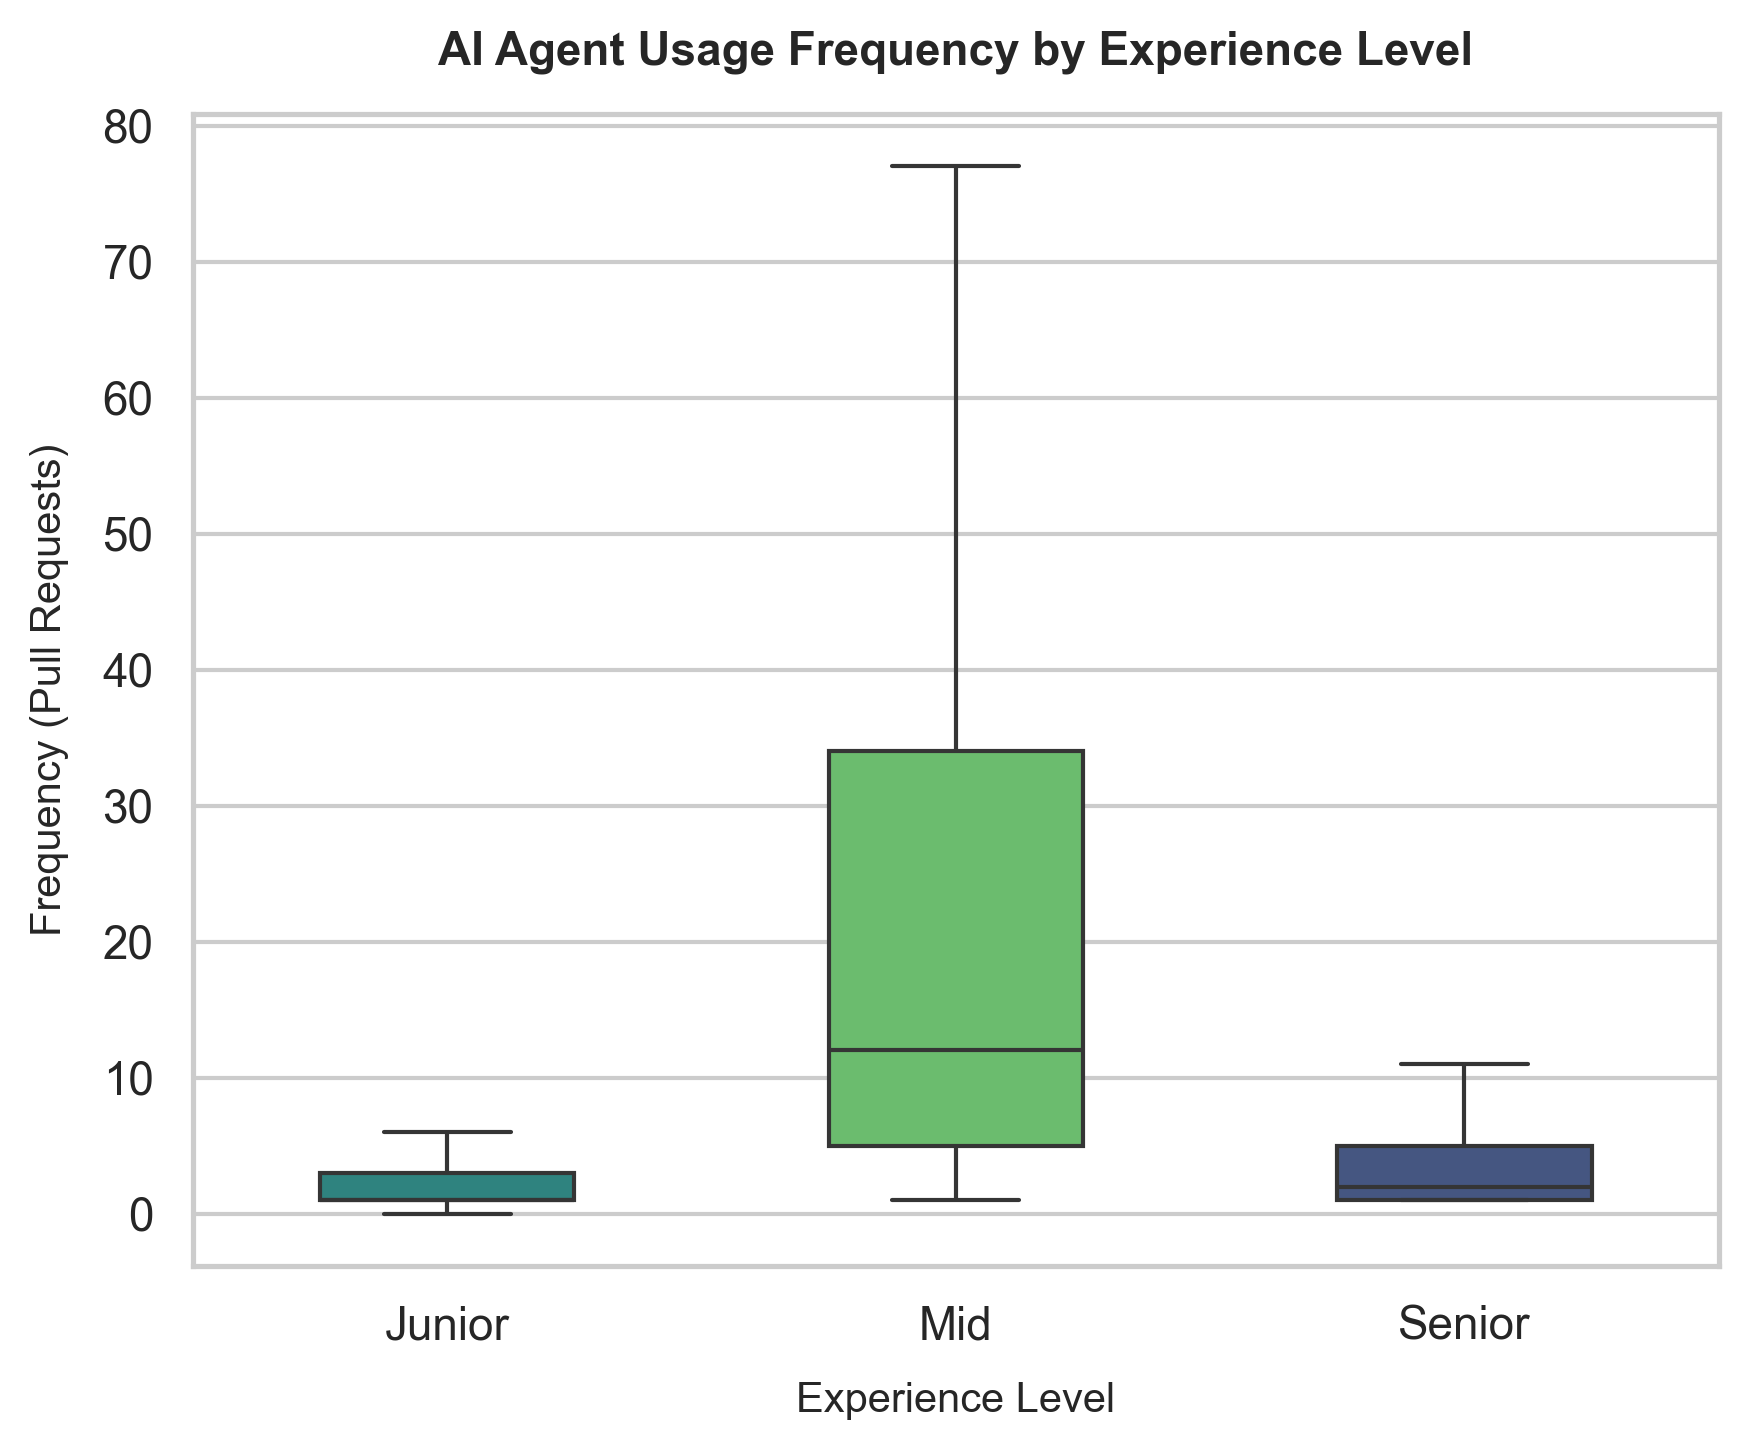
\includegraphics[width=0.85\linewidth]{box_plot.png}
    \label{fig:box_plot-exp1}
\end{figure}

\subsection{RQ2: Does human experience translate into a higher acceptance rate of agent-generated code?}

Table~\ref{tab:rq2-summary} shows the share of resolved Agentic-PRs that were merged, broken down by developer. The Kruskal-Wallis test confirmed a significant difference between profiles ($H = 2380.03$, $p < 10^{-300}$, $\varepsilon^2 = 0.043$, 95\% bootstrap CI $[0.039, 0.046]$). All three pairwise comparisons were significant:
\begin{itemize}
    \item \textbf{Senior vs.\ Junior}: $U = 1.583\times10^{8}$, $p < 10^{-259}$, rank-biserial $r = 0.151$, 95\% CI $[0.142, 0.160]$.
    \item \textbf{Senior vs.\ Mid}: $U = 7.458\times10^{7}$, $p < 10^{-3}$, rank-biserial $r = -0.022$, 95\% CI $[-0.035, -0.009]$.
    \item \textbf{Mid vs.\ Junior}: $U = 1.537\times10^{8}$, $p < 10^{-300}$, rank-biserial $r = 0.210$, 95\% CI $[0.200, 0.219]$.
\end{itemize}

\textbf{Mid has the highest mean acceptance rate (91.8\%), slightly ahead of Junior (90.2\%), with a clearly lowest score for Senior (83.2\%).}

The Senior-Mid effect is statistically significant, but negligible in size ($r = -0.02$); more meaningful are the contrasts showing lower acceptance for Senior compared to both other profiles. This is not the strict, monotonic decrease reported in an earlier version of this analysis, based on clustering that used a quantile transformation (the unstable preprocessing method later replaced with log(1+x) - see Section 3), but the qualitative conclusion stays the same: higher combined activity on GitHub is not associated with a higher acceptance rate for Agentic-PRs - the highest-activity profile has the lowest acceptance in both versions of the analysis.

\begin{table}[H]
    \centering
    \caption{RQ2: Agentic-PR acceptance rate (\%) by activity profile.}
    \label{tab:rq2-summary}
    \small
    \begin{tabular}{lrrrr}
        \toprule
        Profile & $N$ & Mean & Std.\ dev.\ & Median \\
        \midrule
        Junior & 31,522 & 90.20 & 27.04 & 100.0 \\
        Mid    & 12,341 & 91.76 & 18.03 & 100.0 \\
        Senior & 11,830 & 83.18 & 32.50 & 100.0 \\
        \bottomrule
    \end{tabular}
\end{table}

\begin{figure}[H]
    \centering
    
\includegraphics[width=1\linewidth]{second_experiment_box_plot.png}
    \label{fig:boxplot-exp2}
\end{figure}
\subsection{RQ3: How does the acceptance rate of Agentic-PRs compare to a human-authored baseline?}
As described in Section 3, this is a population-level comparison, not one based on activity profiles: the full Agentic-PR population (from RQ2, summed across profiles) compared to the independent \texttt{human\_pull\_request} baseline - so it is not affected by the change in clustering preprocessing. Table~\ref{tab:rq3-summary} shows descriptive statistics for both groups.

A two-sided Mann-Whitney $U$ test showed a statistically significant difference ($U = 6.795 \times 10^{7}$, $p < 10^{-8}$, rank-biserial correlation $r = -0.054$, 95\% bootstrap CI $[-0.075, -0.034]$). Agentic-PRs are accepted slightly more often (88.9\%) than the baseline human population (78.6\%), though the effect size is small, and the baseline human population has a much larger spread (SD 38.8 vs.\ 26.84). This comparison is not matched at the developer level: the two populations overlap in only 351 of the 2515 authors in the human baseline, so the difference reflects two different populations of contributors in two different (though both highly active) parts of GitHub, not a within-person comparison - the same developer both with and without agent involvement.

\begin{table}[H]
    \centering
    \caption{RQ3: pull-request acceptance rate (\%), Agentic-PR compared to the human-authored baseline.}
    \label{tab:rq3-summary}
    \small
    \begin{tabular}{lrrrr}
        \toprule
        Group & $N$ & Mean & Std.\ dev.\ & Median \\
        \midrule
        Agent (Agentic-PR)       & 56,387 & 88.94 & 26.84 & 100.0 \\
        Human (\texttt{human\_pull\_request}) & 2,286  & 78.65 & 38.80 & 100.0 \\
        \bottomrule
    \end{tabular}
\end{table}

\begin{figure}[H]
    \centering
    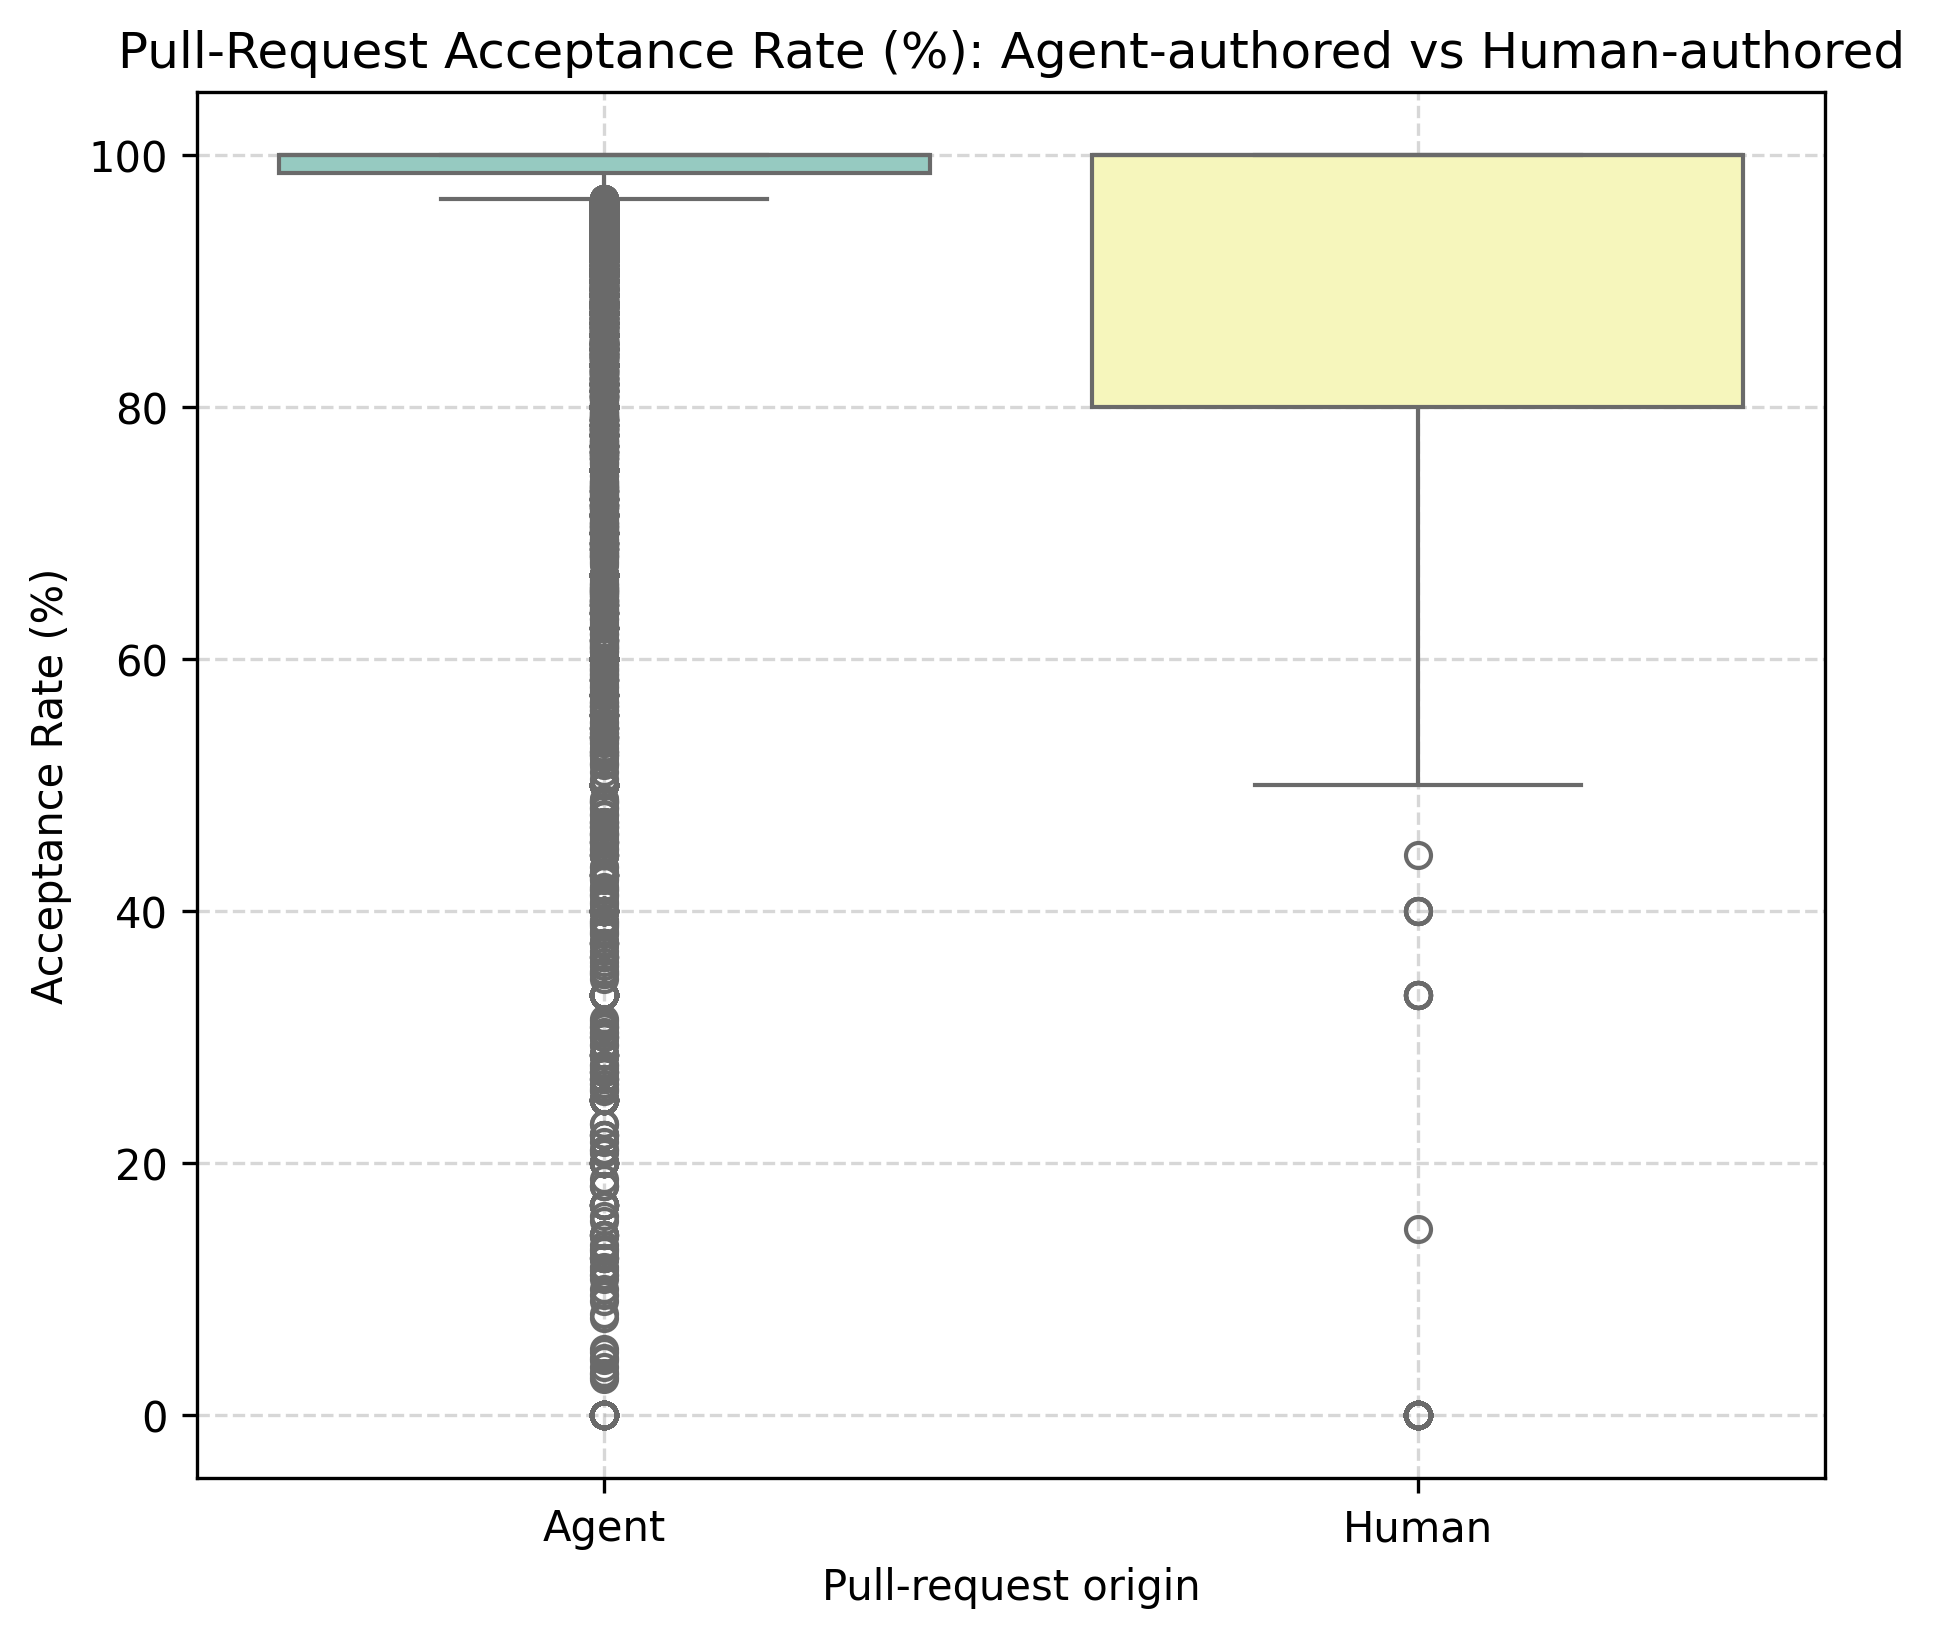
\includegraphics[width=0.85\linewidth]{fourth_experiment_boxplot.png}
    \label{fig:boxplot-exp3}
\end{figure}
